---
class:middle, center
```{tikz}
\usetikzlibrary{calc}\begin{tikzpicture}[scale=4]

\def\delt{0.05}

\coordinate (pt1)  	at (0.0000,0.0000);
\coordinate (pt2)  	at (0.2810,0.1639);
\coordinate (pt3)  	at (0.4009,0.1586);
\coordinate (pt4)  	at (0.4969,0.2385);
\coordinate (pt5)  	at (0.5929,0.1346);
\coordinate (pt6)  	at (0.6489,0.0000);
\coordinate (pt7)  	at (0.7448,-0.132);
\coordinate (pt8)  	at (0.8861,-0.108);
\coordinate (pt9)  	at (0.9714,0.0000);
\coordinate (pt10)  at (1.118,0.0626);
\coordinate (pt11)  at (1.2380,0.0000);

\foreach[evaluate={\finish=int(\start+1)}] \start in {1,2,3,...,10}{
	\draw (pt\start)--(pt\finish);
}

\foreach \num in {1,2,...,11}{
	\draw[fill=orange] (pt\num) circle (0.25pt);
}
\foreach \num in {1,11}{
	\draw[fill=green] (pt\num) circle (0.25pt);
}
\useasboundingbox (-0.1,-0.25) rectangle (1.4,0.35);
\end{tikzpicture}
```
---
class:middle, center
```{tikz}
\usetikzlibrary{calc}
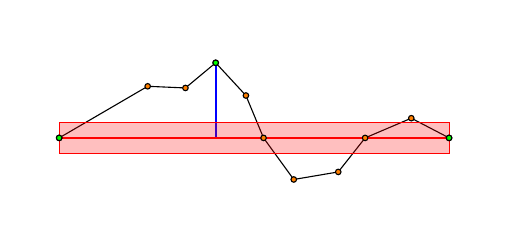
\begin{tikzpicture}[scale=4]


\def\delt{0.05}

\coordinate (pt1)  	at (0.0000,0.0000);
\coordinate (pt2)  	at (0.2810,0.1639);
\coordinate (pt3)  	at (0.4009,0.1586);
\coordinate (pt4)  	at (0.4969,0.2385);
\coordinate (pt5)  	at (0.5929,0.1346);
\coordinate (pt6)  	at (0.6489,0.0000);
\coordinate (pt7)  	at (0.7448,-0.132);
\coordinate (pt8)  	at (0.8861,-0.108);
\coordinate (pt9)  	at (0.9714,0.0000);
\coordinate (pt10)  at (1.118,0.0626);
\coordinate (pt11)  at (1.2380,0.0000);

\foreach[evaluate={\finish=int(\start+1)}] \start in {1,2,3,...,10}{
	\draw (pt\start)--(pt\finish);
}


\draw[blue, thick] (pt1)-|(pt4);
\draw[red, thick] (pt1)--(pt11);
\draw[red, fill opacity=0.25, fill = red] ($(pt1)-(0,\delt)$) rectangle ($(pt11)+(0,\delt)$);

\foreach \num in {1,2,...,11}{
	\draw[fill=orange] (pt\num) circle (0.25pt);
}
\foreach \num in {1,11,4}{
	\draw[fill=green] (pt\num) circle (0.25pt);
}
\useasboundingbox (-0.1,-0.25) rectangle (1.4,0.35);
\end{tikzpicture}
```
---
class:middle, center
```{tikz}
\usetikzlibrary{calc}
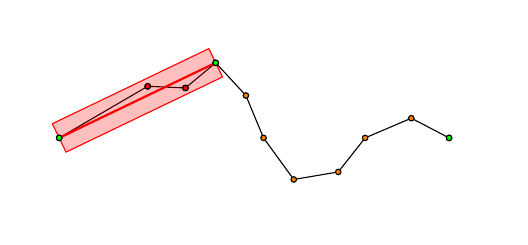
\begin{tikzpicture}[scale=4]


\coordinate (pt1)  	at (0.0000,0.0000);
\coordinate (pt2)  	at (0.2810,0.1639);
\coordinate (pt3)  	at (0.4009,0.1586);
\coordinate (pt4)  	at (0.4969,0.2385);
\coordinate (pt5)  	at (0.5929,0.1346);
\coordinate (pt6)  	at (0.6489,0.0000);
\coordinate (pt7)  	at (0.7448,-0.132);
\coordinate (pt8)  	at (0.8861,-0.108);
\coordinate (pt9)  	at (0.9714,0.0000);
\coordinate (pt10)  at (1.118,0.0626);
\coordinate (pt11)  at (1.2380,0.0000);

\def\delt{0.05cm}

\foreach[evaluate={\finish=int(\start+1)}] \start in {1,2,3,...,10}{
	\draw (pt\start)--(pt\finish);
}

\draw[red, thick] (pt1)--(pt4);

\draw[red, fill = red, fill opacity = 0.25] let \p{A}=(pt1), \p{B}=(pt4) in
	({\x{A}+(\delt/(1+((\x{B}-\x{A})/(\y{B}-\y{A}))^2)^(1/2))},
	 {\y{A}-(\delt/(1+((\x{B}-\x{A})/(\y{B}-\y{A}))^2)^(1/2))*((\x{B}-\x{A})/(\y{B}-\y{A}))})
	 --
	 ({\x{B}+(\delt/(1+((\x{B}-\x{A})/(\y{B}-\y{A}))^2)^(1/2))},
	 {\y{B}-(\delt/(1+((\x{B}-\x{A})/(\y{B}-\y{A}))^2)^(1/2))*((\x{B}-\x{A})/(\y{B}-\y{A}))})
	 --
	 ({\x{B}-(\delt/(1+((\x{B}-\x{A})/(\y{B}-\y{A}))^2)^(1/2))},
	 {\y{B}+(\delt/(1+((\x{B}-\x{A})/(\y{B}-\y{A}))^2)^(1/2))*((\x{B}-\x{A})/(\y{B}-\y{A}))})
	 --
	 ({\x{A}-(\delt/(1+((\x{B}-\x{A})/(\y{B}-\y{A}))^2)^(1/2))},
	 {\y{A}+(\delt/(1+((\x{B}-\x{A})/(\y{B}-\y{A}))^2)^(1/2))*((\x{B}-\x{A})/(\y{B}-\y{A}))})
	 --cycle;

\foreach \num in {1,2,...,11}{
	\draw[fill=orange] (pt\num) circle (0.25pt);
}
\foreach \num in {1,11,4}{
	\draw[fill=green] (pt\num) circle (0.25pt);
}
\foreach \num in {2,3}{
	\draw[fill=red] (pt\num) circle (0.25pt);
}
\useasboundingbox (-0.1,-0.25) rectangle (1.4,0.35);
\end{tikzpicture}
```
---
class:middle, center
```{tikz}
\usetikzlibrary{calc}
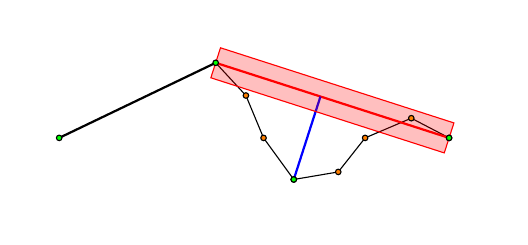
\begin{tikzpicture}[scale=4]


\coordinate (pt1)  	at (0.0000,0.0000);
\coordinate (pt2)  	at (0.2810,0.1639);
\coordinate (pt3)  	at (0.4009,0.1586);
\coordinate (pt4)  	at (0.4969,0.2385);
\coordinate (pt5)  	at (0.5929,0.1346);
\coordinate (pt6)  	at (0.6489,0.0000);
\coordinate (pt7)  	at (0.7448,-0.132);
\coordinate (pt8)  	at (0.8861,-0.108);
\coordinate (pt9)  	at (0.9714,0.0000);
\coordinate (pt10)  at (1.118,0.0626);
\coordinate (pt11)  at (1.2380,0.0000);

\def\delt{0.05cm}

\foreach[evaluate={\finish=int(\start+1)}] \start in {4,5,6,...,10}{
	\draw (pt\start)--(pt\finish);
}

\draw[thick] (pt1)--(pt4);
\draw[red, thick] (pt4)--(pt11);

\draw[blue, thick] let \p{A}=(pt4), \p{B}=(pt11), \p{P}=(pt7) in
	(pt7)--
	({\x{A}+(\x{B}-\x{A})*((\x{P}-\x{A})*(\x{B}-\x{A})+(\y{P}-\y{A})*(\y{B}-\y{A}))/((\x{B}-\x{A})^2+(\y{B}-\y{A})^2)},
	{\y{A}+(\y{B}-\y{A})*((\x{P}-\x{A})*(\x{B}-\x{A})+(\y{P}-\y{A})*(\y{B}-\y{A}))/((\x{B}-\x{A})^2+(\y{B}-\y{A})^2)});

\draw[red, fill = red, fill opacity = 0.25] let \p{A}=(pt4), \p{B}=(pt11) in
	({\x{A}+(\delt/(1+((\x{B}-\x{A})/(\y{B}-\y{A}))^2)^(1/2))},
	 {\y{A}-(\delt/(1+((\x{B}-\x{A})/(\y{B}-\y{A}))^2)^(1/2))*((\x{B}-\x{A})/(\y{B}-\y{A}))})
	 --
	 ({\x{B}+(\delt/(1+((\x{B}-\x{A})/(\y{B}-\y{A}))^2)^(1/2))},
	 {\y{B}-(\delt/(1+((\x{B}-\x{A})/(\y{B}-\y{A}))^2)^(1/2))*((\x{B}-\x{A})/(\y{B}-\y{A}))})
	 --
	 ({\x{B}-(\delt/(1+((\x{B}-\x{A})/(\y{B}-\y{A}))^2)^(1/2))},
	 {\y{B}+(\delt/(1+((\x{B}-\x{A})/(\y{B}-\y{A}))^2)^(1/2))*((\x{B}-\x{A})/(\y{B}-\y{A}))})
	 --
	 ({\x{A}-(\delt/(1+((\x{B}-\x{A})/(\y{B}-\y{A}))^2)^(1/2))},
	 {\y{A}+(\delt/(1+((\x{B}-\x{A})/(\y{B}-\y{A}))^2)^(1/2))*((\x{B}-\x{A})/(\y{B}-\y{A}))})
	 --cycle;

\foreach \num in {5,6,...,11}{
	\draw[fill=orange] (pt\num) circle (0.25pt);
}
\foreach \num in {1,11,4,7}{
	\draw[fill=green] (pt\num) circle (0.25pt);
}
\useasboundingbox (-0.1,-0.25) rectangle (1.4,0.35);
\end{tikzpicture}
```
---
class:middle, center
```{tikz}
\usetikzlibrary{calc}
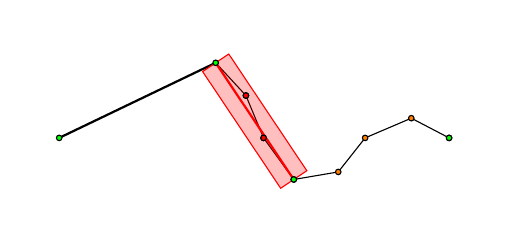
\begin{tikzpicture}[scale=4]


\coordinate (pt1)  	at (0.0000,0.0000);
\coordinate (pt2)  	at (0.2810,0.1639);
\coordinate (pt3)  	at (0.4009,0.1586);
\coordinate (pt4)  	at (0.4969,0.2385);
\coordinate (pt5)  	at (0.5929,0.1346);
\coordinate (pt6)  	at (0.6489,0.0000);
\coordinate (pt7)  	at (0.7448,-0.132);
\coordinate (pt8)  	at (0.8861,-0.108);
\coordinate (pt9)  	at (0.9714,0.0000);
\coordinate (pt10)  at (1.118,0.0626);
\coordinate (pt11)  at (1.2380,0.0000);

\def\delt{0.05cm}

\foreach[evaluate={\finish=int(\start+1)}] \start in {4,5,6,...,10}{
	\draw (pt\start)--(pt\finish);
}

\draw[thick] (pt1)--(pt4);
\draw[red, thick] (pt4)--(pt7);

\draw[red, fill = red, fill opacity = 0.25] let \p{A}=(pt4), \p{B}=(pt7) in
	({\x{A}+(\delt/(1+((\x{B}-\x{A})/(\y{B}-\y{A}))^2)^(1/2))},
	 {\y{A}-(\delt/(1+((\x{B}-\x{A})/(\y{B}-\y{A}))^2)^(1/2))*((\x{B}-\x{A})/(\y{B}-\y{A}))})
	 --
	 ({\x{B}+(\delt/(1+((\x{B}-\x{A})/(\y{B}-\y{A}))^2)^(1/2))},
	 {\y{B}-(\delt/(1+((\x{B}-\x{A})/(\y{B}-\y{A}))^2)^(1/2))*((\x{B}-\x{A})/(\y{B}-\y{A}))})
	 --
	 ({\x{B}-(\delt/(1+((\x{B}-\x{A})/(\y{B}-\y{A}))^2)^(1/2))},
	 {\y{B}+(\delt/(1+((\x{B}-\x{A})/(\y{B}-\y{A}))^2)^(1/2))*((\x{B}-\x{A})/(\y{B}-\y{A}))})
	 --
	 ({\x{A}-(\delt/(1+((\x{B}-\x{A})/(\y{B}-\y{A}))^2)^(1/2))},
	 {\y{A}+(\delt/(1+((\x{B}-\x{A})/(\y{B}-\y{A}))^2)^(1/2))*((\x{B}-\x{A})/(\y{B}-\y{A}))})
	 --cycle;

\foreach \num in {5,6,...,11}{
	\draw[fill=orange] (pt\num) circle (0.25pt);
}
\foreach \num in {1,11,4,7}{
	\draw[fill=green] (pt\num) circle (0.25pt);
}
\foreach \num in {5,6}{
	\draw[fill=red] (pt\num) circle (0.25pt);
}
\useasboundingbox (-0.1,-0.25) rectangle (1.4,0.35);
\end{tikzpicture}
```
---
class:middle, center
```{tikz}
\usetikzlibrary{calc}
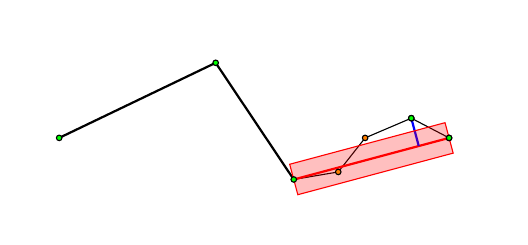
\begin{tikzpicture}[scale=4]


\coordinate (pt1)  	at (0.0000,0.0000);
\coordinate (pt2)  	at (0.2810,0.1639);
\coordinate (pt3)  	at (0.4009,0.1586);
\coordinate (pt4)  	at (0.4969,0.2385);
\coordinate (pt5)  	at (0.5929,0.1346);
\coordinate (pt6)  	at (0.6489,0.0000);
\coordinate (pt7)  	at (0.7448,-0.132);
\coordinate (pt8)  	at (0.8861,-0.108);
\coordinate (pt9)  	at (0.9714,0.0000);
\coordinate (pt10)  at (1.118,0.0626);
\coordinate (pt11)  at (1.2380,0.0000);

\def\delt{0.05cm}

\foreach[evaluate={\finish=int(\start+1)}] \start in {7,8,9,...,10}{
	\draw (pt\start)--(pt\finish);
}

\draw[thick] (pt1)--(pt4)--(pt7);
\draw[red, thick] (pt7)--(pt11);

\draw[blue, thick] let \p{A}=(pt7), \p{B}=(pt11), \p{P}=(pt10) in
	(\x{P},\y{P})--
	({\x{A}+(\x{B}-\x{A})*((\x{P}-\x{A})*(\x{B}-\x{A})+(\y{P}-\y{A})*(\y{B}-\y{A}))/((\x{B}-\x{A})^2+(\y{B}-\y{A})^2)},
	{\y{A}+(\y{B}-\y{A})*((\x{P}-\x{A})*(\x{B}-\x{A})+(\y{P}-\y{A})*(\y{B}-\y{A}))/((\x{B}-\x{A})^2+(\y{B}-\y{A})^2)});

\draw[red, fill = red, fill opacity = 0.25] let \p{A}=(pt7), \p{B}=(pt11) in
	({\x{A}+(\delt/(1+((\x{B}-\x{A})/(\y{B}-\y{A}))^2)^(1/2))},
	 {\y{A}-(\delt/(1+((\x{B}-\x{A})/(\y{B}-\y{A}))^2)^(1/2))*((\x{B}-\x{A})/(\y{B}-\y{A}))})
	 --
	 ({\x{B}+(\delt/(1+((\x{B}-\x{A})/(\y{B}-\y{A}))^2)^(1/2))},
	 {\y{B}-(\delt/(1+((\x{B}-\x{A})/(\y{B}-\y{A}))^2)^(1/2))*((\x{B}-\x{A})/(\y{B}-\y{A}))})
	 --
	 ({\x{B}-(\delt/(1+((\x{B}-\x{A})/(\y{B}-\y{A}))^2)^(1/2))},
	 {\y{B}+(\delt/(1+((\x{B}-\x{A})/(\y{B}-\y{A}))^2)^(1/2))*((\x{B}-\x{A})/(\y{B}-\y{A}))})
	 --
	 ({\x{A}-(\delt/(1+((\x{B}-\x{A})/(\y{B}-\y{A}))^2)^(1/2))},
	 {\y{A}+(\delt/(1+((\x{B}-\x{A})/(\y{B}-\y{A}))^2)^(1/2))*((\x{B}-\x{A})/(\y{B}-\y{A}))})
	 --cycle;

\foreach \num in {8,9,10,11}{
	\draw[fill=orange] (pt\num) circle (0.25pt);
}
\foreach \num in {1,11,4,7, 10}{
	\draw[fill=green] (pt\num) circle (0.25pt);
}
\useasboundingbox (-0.1,-0.25) rectangle (1.4,0.35);
\end{tikzpicture}
```
---
class:middle, center
```{tikz}
\usetikzlibrary{calc}
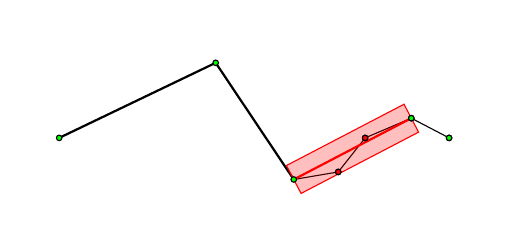
\begin{tikzpicture}[scale=4]


\coordinate (pt1)  	at (0.0000,0.0000);
\coordinate (pt2)  	at (0.2810,0.1639);
\coordinate (pt3)  	at (0.4009,0.1586);
\coordinate (pt4)  	at (0.4969,0.2385);
\coordinate (pt5)  	at (0.5929,0.1346);
\coordinate (pt6)  	at (0.6489,0.0000);
\coordinate (pt7)  	at (0.7448,-0.132);
\coordinate (pt8)  	at (0.8861,-0.108);
\coordinate (pt9)  	at (0.9714,0.0000);
\coordinate (pt10)  at (1.118,0.0626);
\coordinate (pt11)  at (1.2380,0.0000);

\def\delt{0.05cm}

\foreach[evaluate={\finish=int(\start+1)}] \start in {7,8,9,...,10}{
	\draw (pt\start)--(pt\finish);
}

\draw[thick] (pt1)--(pt4)--(pt7);
\draw[red, thick] (pt7)--(pt10);

\draw[red, fill = red, fill opacity = 0.25] let \p{A}=(pt7), \p{B}=(pt10) in
	({\x{A}+(\delt/(1+((\x{B}-\x{A})/(\y{B}-\y{A}))^2)^(1/2))},
	 {\y{A}-(\delt/(1+((\x{B}-\x{A})/(\y{B}-\y{A}))^2)^(1/2))*((\x{B}-\x{A})/(\y{B}-\y{A}))})
	 --
	 ({\x{B}+(\delt/(1+((\x{B}-\x{A})/(\y{B}-\y{A}))^2)^(1/2))},
	 {\y{B}-(\delt/(1+((\x{B}-\x{A})/(\y{B}-\y{A}))^2)^(1/2))*((\x{B}-\x{A})/(\y{B}-\y{A}))})
	 --
	 ({\x{B}-(\delt/(1+((\x{B}-\x{A})/(\y{B}-\y{A}))^2)^(1/2))},
	 {\y{B}+(\delt/(1+((\x{B}-\x{A})/(\y{B}-\y{A}))^2)^(1/2))*((\x{B}-\x{A})/(\y{B}-\y{A}))})
	 --
	 ({\x{A}-(\delt/(1+((\x{B}-\x{A})/(\y{B}-\y{A}))^2)^(1/2))},
	 {\y{A}+(\delt/(1+((\x{B}-\x{A})/(\y{B}-\y{A}))^2)^(1/2))*((\x{B}-\x{A})/(\y{B}-\y{A}))})
	 --cycle;

\foreach \num in {8,9,10,11}{
	\draw[fill=orange] (pt\num) circle (0.25pt);
}
\foreach \num in {1,11,4,7, 10}{
	\draw[fill=green] (pt\num) circle (0.25pt);
}
\foreach \num in {8,9}{
	\draw[fill=red] (pt\num) circle (0.25pt);
}
\useasboundingbox (-0.1,-0.25) rectangle (1.4,0.35);
\end{tikzpicture}
```
---
class:middle, center
```{tikz}
\usetikzlibrary{calc}
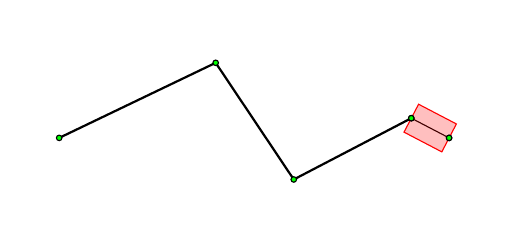
\begin{tikzpicture}[scale=4]


\coordinate (pt1)  	at (0.0000,0.0000);
\coordinate (pt2)  	at (0.2810,0.1639);
\coordinate (pt3)  	at (0.4009,0.1586);
\coordinate (pt4)  	at (0.4969,0.2385);
\coordinate (pt5)  	at (0.5929,0.1346);
\coordinate (pt6)  	at (0.6489,0.0000);
\coordinate (pt7)  	at (0.7448,-0.132);
\coordinate (pt8)  	at (0.8861,-0.108);
\coordinate (pt9)  	at (0.9714,0.0000);
\coordinate (pt10)  at (1.118,0.0626);
\coordinate (pt11)  at (1.2380,0.0000);

\def\delt{0.05cm}

\draw (pt10)--(pt11);
\draw[thick] (pt1)--(pt4)--(pt7)--(pt10);

\draw[red, fill = red, fill opacity = 0.25] let \p{A}=(pt10), \p{B}=(pt11) in
	({\x{A}+(\delt/(1+((\x{B}-\x{A})/(\y{B}-\y{A}))^2)^(1/2))},
	 {\y{A}-(\delt/(1+((\x{B}-\x{A})/(\y{B}-\y{A}))^2)^(1/2))*((\x{B}-\x{A})/(\y{B}-\y{A}))})
	 --
	 ({\x{B}+(\delt/(1+((\x{B}-\x{A})/(\y{B}-\y{A}))^2)^(1/2))},
	 {\y{B}-(\delt/(1+((\x{B}-\x{A})/(\y{B}-\y{A}))^2)^(1/2))*((\x{B}-\x{A})/(\y{B}-\y{A}))})
	 --
	 ({\x{B}-(\delt/(1+((\x{B}-\x{A})/(\y{B}-\y{A}))^2)^(1/2))},
	 {\y{B}+(\delt/(1+((\x{B}-\x{A})/(\y{B}-\y{A}))^2)^(1/2))*((\x{B}-\x{A})/(\y{B}-\y{A}))})
	 --
	 ({\x{A}-(\delt/(1+((\x{B}-\x{A})/(\y{B}-\y{A}))^2)^(1/2))},
	 {\y{A}+(\delt/(1+((\x{B}-\x{A})/(\y{B}-\y{A}))^2)^(1/2))*((\x{B}-\x{A})/(\y{B}-\y{A}))})
	 --cycle;

\foreach \num in {10,11}{
	\draw[fill=orange] (pt\num) circle (0.25pt);
}
\foreach \num in {1,11,4,7, 10}{
	\draw[fill=green] (pt\num) circle (0.25pt);
}
\useasboundingbox (-0.1,-0.25) rectangle (1.4,0.35);
\end{tikzpicture}
```
---
class:middle, center
```{tikz}
\usetikzlibrary{calc}
\begin{tikzpicture}[scale=4]


\coordinate (pt1)  	at (0.0000,0.0000);
\coordinate (pt2)  	at (0.2810,0.1639);
\coordinate (pt3)  	at (0.4009,0.1586);
\coordinate (pt4)  	at (0.4969,0.2385);
\coordinate (pt5)  	at (0.5929,0.1346);
\coordinate (pt6)  	at (0.6489,0.0000);
\coordinate (pt7)  	at (0.7448,-0.132);
\coordinate (pt8)  	at (0.8861,-0.108);
\coordinate (pt9)  	at (0.9714,0.0000);
\coordinate (pt10)  at (1.118,0.0626);
\coordinate (pt11)  at (1.2380,0.0000);

\def\delt{0.05cm}

\draw[thick] (pt1)--(pt4)--(pt7)--(pt10)--(pt11);

\foreach \num in {10,11}{
	\draw[fill=orange] (pt\num) circle (0.25pt);
}
\foreach \num in {1,11,4,7, 10}{
	\draw[fill=green] (pt\num) circle (0.25pt);
}
\useasboundingbox (-0.1,-0.25) rectangle (1.4,0.35);
\end{tikzpicture}
```
